\documentclass{sig-alternate-05-2015}
\usepackage{graphicx}
\usepackage{caption}
\usepackage{subcaption}


\newenvironment{myitemize}{\begin{itemize} \setlength{\topsep}{0pt} \setlength{\itemsep}{0pt} \setlength{\parskip}{0pt} \setlength{\parsep}{0pt}}{  \end{itemize} }

\setlength{\itemsep}{0pt}

\begin{document}

% Copyright
\CopyrightYear{2016} 
\setcopyright{rightsretained} 
\conferenceinfo{RecSys '16}{September 15-19, 2016, Boston , MA, USA} 
\isbn{978-1-4503-4035-9/16/09}
\doi{http://dx.doi.org/10.1145/2959100.2959207}

\clubpenalty=10000 
\widowpenalty = 10000


\title{RecSys Challenge 2016: Job Recommendations}

% Authors (in alphabetical order):
\numberofauthors{5} 

\author{
\alignauthor
Fabian Abel\\
       \affaddr{XING AG}\\
       \affaddr{Hamburg, Germany}\\
       \affaddr{fabian.abel@xing.com}
\alignauthor
Andr�s Bencz�r\\
       \affaddr{Hungarian Academy of Sciences}\\
       \affaddr{Budapest, Hungary}\\
       \affaddr{benczur@sztaki.hu}
\and
Daniel Kohlsdorf\\
       \affaddr{XING AG}\\
       \affaddr{Hamburg, Germany}\\
       \affaddr{daniel.kohlsdorf@xing.com}
\alignauthor 
Martha Larson\\
       \affaddr{TU Delft}\\
       \affaddr{Delft, Netherlands}\\
       \affaddr{m.a.larson@tudelft.nl}
\alignauthor 
R�bert P�lovics\\
       \affaddr{Hungarian Academy of Sciences}\\
       \affaddr{Budapest, Hungary}\\
       \affaddr{palovics@sztaki.hu}
}

\maketitle
\begin{abstract}
The 2016 ACM Recommender Systems Challenge focused on the problem of job recommendations.
Given a large dataset from XING that consisted of anonymized user profiles, job postings, and interactions between them, the participating teams had to predict job postings that a user will interact with. 

The challenge ran for four months with a final 366 registered teams.
The number of active teams were 119 and they have submitted together 4232 solutions yielding in an impressive neck-and-neck race that was decided within the last days of the challenge.
\end{abstract}


%
% The code below should be generated by the tool at
% http://dl.acm.org/ccs.cfm
% Please copy and paste the code instead of the example below. 
%
\begin{CCSXML}
<ccs2012>
<concept>
<concept_id>10002951.10003317.10003347.10003350</concept_id>
<concept_desc>Information systems~Recommender systems</concept_desc>
<concept_significance>500</concept_significance>
</concept>
<concept>
<concept_id>10002951.10003227.10003351</concept_id>
<concept_desc>Information systems~Data mining</concept_desc>
<concept_significance>300</concept_significance>
</concept>
<concept>
<concept_id>10002951.10003317.10003359.10003360</concept_id>
<concept_desc>Information systems~Test collections</concept_desc>
<concept_significance>300</concept_significance>
</concept>
</ccs2012>
\end{CCSXML}

\ccsdesc[500]{Information systems~Recommender systems}
\ccsdesc[300]{Information systems~Data mining}
\ccsdesc[300]{Information systems~Test collections}


%
% End generated code
%

%
%  Use this command to print the description
%
\printccsdesc

% We no longer use \terms command
%\terms{Theory}

\keywords{Recommender Systems; Data Mining Challenge; XING; Job Recommendation}

\section{Introduction}
The ACM RecSys Challenge allows researchers and engineers around the 
world to jointly work on real-world recommender system problems in various domains such as social media related recommendations~\cite{recsyschallenge:2014} or product recommendations~\cite{recsyschallenge:2015}. 
In 2016, the challenge was dedicated to the problem of job recommendation\footnote{\url{http://2016.recsyschallenge.com}}~\cite{job:recommendations}. 
We released a large dataset from XING\footnote{\url{http://xing.com}} that is a business-oriented social network with around 18~Million users world-wide and more than 10~Million users in Germany. 

XING supports people in discovering career opportunities, hence the job recommendation system is an essential part of the XING platform.
The provided recommendations aim to satisfy the demands of both the job seekers who have certain preferences concerning their next career step and the recruiters who aim to hire the most appropriate candidate for a given job.
In this challenge, we focused on the demands of the job seekers by defining the following task.

{\em Given a XING user, the recommender had to predict those job postings that a user will positively interact with by clicking on it or bookmarking it.}

  
\section{Dataset}
\begin{figure}
\centering
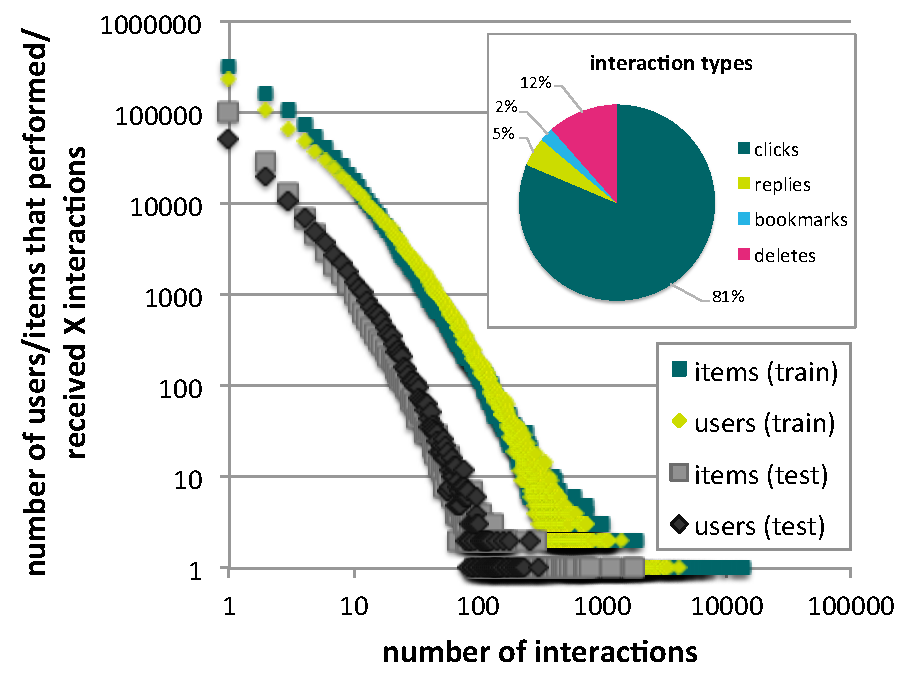
\includegraphics[width=0.45\textwidth]{data-interactions-combined.pdf}
\vspace{-0.3cm}
\caption{Number of interactions per user and item. 328,618 items (24.2\%) and 582,370 users (42.9\%) remained without interactions during the training period. More than 80\% of the interactions are clicks, followed by deletes, replies and bookmarks. The distributions for training data and test data (ground truth) follow similar characteristics.}
\label{fig:data-interactions}
\end{figure}

\begin{figure*}[t]
    \centering
    \begin{subfigure}[t]{0.3\textwidth}
        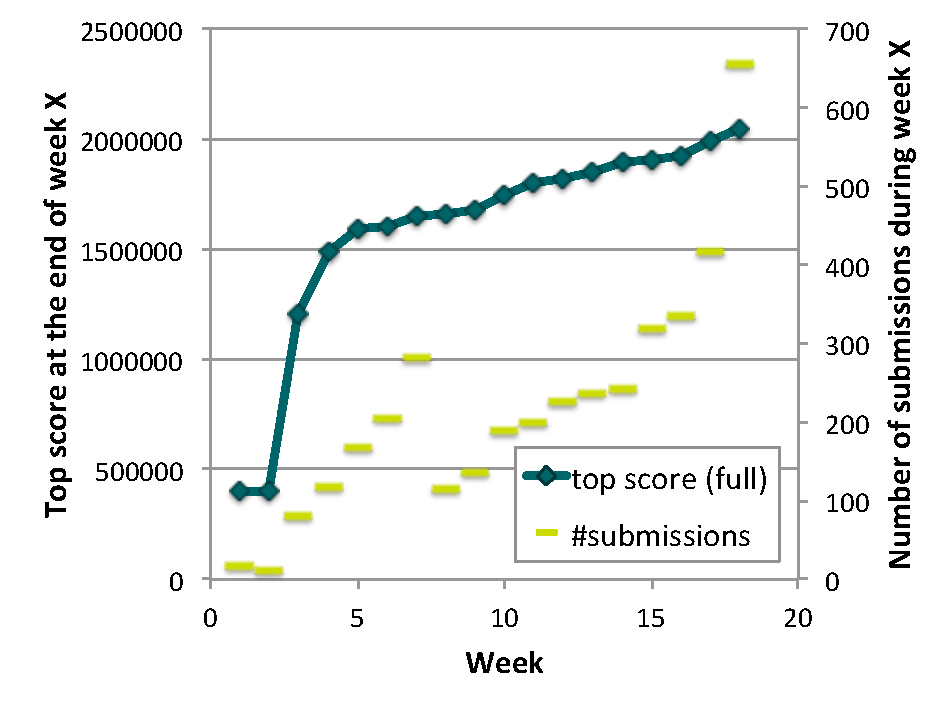
\includegraphics[width=\textwidth]{results-top-score-over-time.pdf}
  \caption{Top score over time and number of submissions during each week of the challenge.}
  \label{fig:results-scores-over-time}
    \end{subfigure}
    ~ %add desired spacing between images, e. g. ~, \quad, \qquad, \hfill etc. 
      %(or a blank line to force the subfigure onto a new line)
    \begin{subfigure}[t]{0.3\textwidth}
  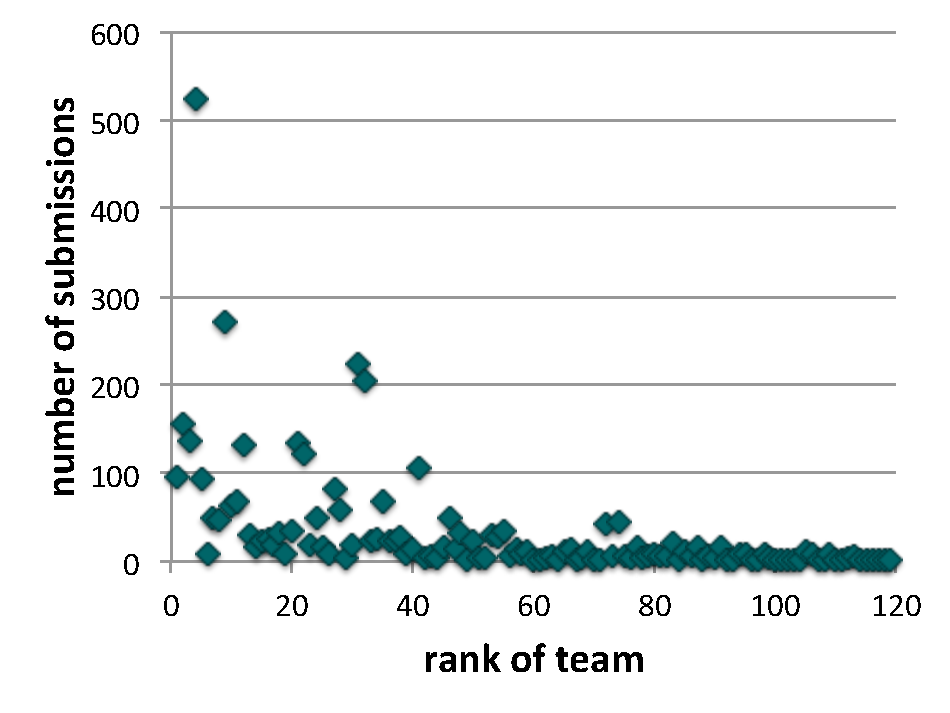
\includegraphics[width=\textwidth]{results-submissions-by-rank.pdf}
  \caption{Number of submissions per team (ordered by final rank of the team).}
  \label{fig:results-submissions-by-rank}
    \end{subfigure}
    ~ %add desired spacing between images, e. g. ~, \quad, \qquad, \hfill etc. 
    %(or a blank line to force the subfigure onto a new line)
    \begin{subfigure}[t]{0.3\textwidth}
  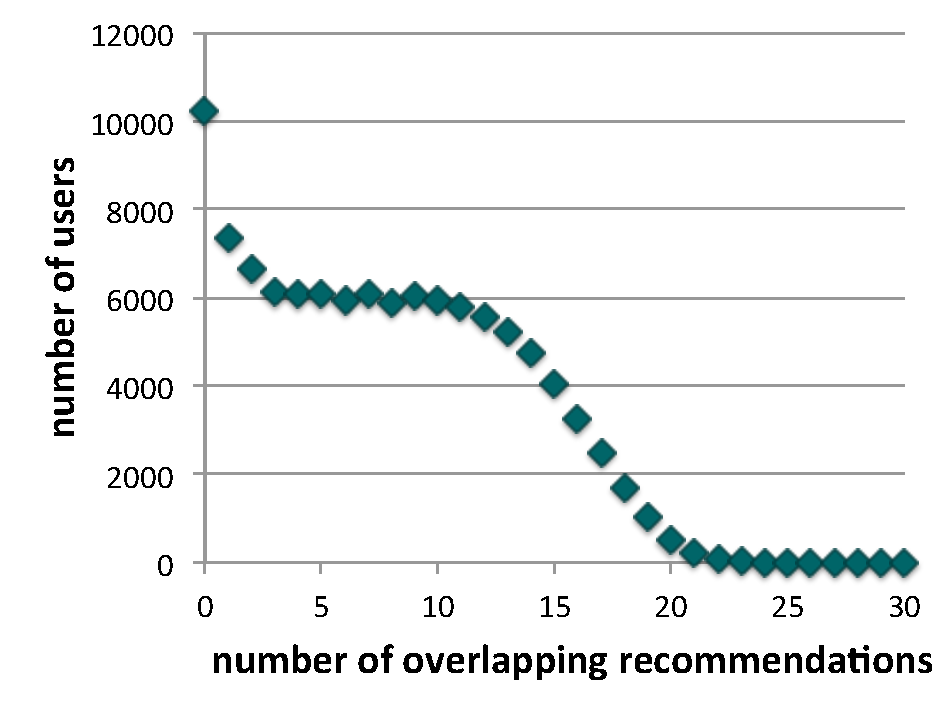
\includegraphics[width=\textwidth]{results-overlap-with-xing-recos.pdf}
  \caption{Overlap between top solution and recommendations generated by XING's job recommender.}
  \label{fig:results-overlap-xing}
    \end{subfigure}
    \caption{Submission statistics.}\label{fig:results}
\end{figure*}

We provided a training dataset featuring user profiles, job postings, and interactions that users performed on job posts.
The dataset also incorporated user-item impressions: we released information about job postings that were shown to users in the XING platform.
The training data\footnote{\url{https://github.com/recsyschallenge/2016/}} contained 1,367,057 users and 1,358,098 items. 
Users and items were described by several similar attributes such as job categories, career level, industry, location, etc.
In addition, the educational background and details about work experience were given for the users. 

Around 12 weeks of implicit interaction data between the users and the items was released for training including
\begin{myitemize}
\item user clicks on job postings, 
\item bookmarks indicating that a user was intended in a given job and saved it for later,
\item replies indicating that a user intended to apply for the job, and
\item deletes when the user removed an item that was irrelevant for her.
\end{myitemize}
Figure~\ref{fig:data-interactions} describes the characteristics of the different interactions.
Two weeks of interactions for a set of 150,000 \emph{target users} were used as test data in order to evaluate the submitted solutions. 
Figure~\ref{fig:data-interactions} also shows the distribution of that ground truth dataset. 


\subsection{Anonymization}
The training dataset is a semi-synthetic sample of XING data. The dataset was designed 
to retain information that is useful for the participants in creating effective algorithms 
that address the challenge, while at the same time protecting the privacy of XING users. 
The data set is semi-synthetic in that it is enriched with artificial users whose presence 
contributes to the anonymization.

The dataset contains, for example, artificial users which were generated by clustering real 
users. Moreover, it contains only a fraction of XING users and job postings and 
not necessarily all interactions of a user were exported. Instead of releasing raw attribute values, 
we performed named entity recognition (e.g. for skills, job roles) and mapped raw strings to IDs 
(pseudonymization). Synonyms such as "Java Software Developer" or "Java Software Engineer" 
wer mapped to the same ID. For some of the users, we removed some of the attribute values 
to further anonymise their profiles. All timestamps in the dataset were shifted by a couple 
of weeks. The sequential order of the interactions was however not changed. 


\section{Challenge Setup and Results}
We used a scoring function as evaluation measure that combines precision@k and recall@k. 
This evaluation measure was based on the key performance indicators that XING is 
using to monitor the quality of the job recommender system. 
Each team was allowed to submit 5~solutions per day and solution files were allowed to 
feature at maximum 30~recommendations per user. A public leaderboard which was based on 
30\% of the ground truth data immediately informed the teams about the performance of their 
algorithms. 

The participating teams came from more than 30~different countries such as USA (25\%), Germany (11\%), 
China (9\%), France (7\%) or Hungary (4\%). Teams came from both academia ($\sim$25\%) and 
industry ($\sim$75\%, most common industry: \textit{Internet \& IT}), e.g. from larger companies such 
as Yandex, Alibaba, Microsoft or Amazon as well as from smaller start-up companies. 

The evolution of the top full score---based on the entire ground truth---is depicted 
in Figure~\ref{fig:results-scores-over-time} together with the number of submissions that 
were performed during that week. The top score thus increased from week to week. In fact, the 
highest score of the challenge was achieved just 30~minutes before the official submission deadline.
Figure~\ref{fig:results-submissions-by-rank} reveals that not only the top teams very highly active 
in submitting solutions but also many teams that finally ended up at rank 30 and above 
submitted a high number of solutions. 

The top solution achieved a score of 2,052,185 points which corresponds to 24.1\% of the 
best possible score.
% and is already close to XING's job recommendation system which scores around 3~Million points. 
Figure~\ref{fig:results-overlap-xing} shows moreover that the 
top solution also manages to recommend items that XING's recommender system does not 
recommend. Hence, the algorithms developed during the challenge seem to complement 
XING's recommender ensemble and are likely to have 
a significant impact on XING's job recommendations. 


\section*{Acknowledgments}
{\small
The work leading to these results has received funding from the EU's 
Seventh Framework Programme (FP7/2007-2013) under CrowdRec
Grant Agreement no.~610594.

% \bibliographystyle{abbrv}
% \bibliography{sigproc}  % sigproc.bib is the name of the Bibliography in this case
\begin{thebibliography}{1}

\bibitem{job:recommendations}
F.~Abel.
\newblock We know where you should work next summer: Job recommendations.
\newblock In {\em Proceedings of the 9th ACM Conference on Recommender
  Systems}, RecSys '15, pages 230--230, New York, NY, USA, 2015. ACM.

\bibitem{recsyschallenge:2015}
D.~Ben-Shimon, A.~Tsikinovsky, M.~Friedmann, B.~Shapira, L.~Rokach, and
  J.~Hoerle.
\newblock Recsys challenge 2015 and the yoochoose dataset.
\newblock In {\em Proceedings of the 9th ACM Conference on Recommender
  Systems}, RecSys '15, pages 357--358, New York, NY, USA, 2015. ACM.

\bibitem{recsyschallenge:2014}
A.~Said, S.~Dooms, B.~Loni, and D.~Tikk.
\newblock Recommender systems challenge 2014.
\newblock In {\em Proceedings of the 8th ACM Conference on Recommender
  Systems}, RecSys '14, pages 387--388, New York, NY, USA, 2014. ACM.
\end{thebibliography}
}
\end{document}
